\textbf{Software Testing }
%WARUM SOLLTE GETESTET WERDEN´?
%WIESO END2END UND UNIT TEST?
%PROJEKTE SCHREITERN WEGEN MANGELHAFTE TESTING \%

In den letzten x Jahren hat das Software-Testing an Bedeutung gewonnen, unter anderem weil man erkannt hat, dass die Kosten für das Überspringen von Testaktivitäten sehr hoch sein können. Unternehmen waren gezwungen, ihren Betrieb zu unterbrechen, und haben aufgrund von Fehlern in ihren Anwendungen Kunden verloren. [BEISPIELE/QUELLE].
Beispiele dazu finden in den Fällen von...: 
Nissan musste für... und COP hat xx verloren(Geld) für....
Neben der Verringerung des Risikos der oben genannten Situationen bietet das Software-Testing weitere Vorteile. Durch das Testing ...
Um einige Vorteile zu nennen: Es wird qualitativ hochwertigerer Code erstellt, Verringerung der Wahrscheinlichkeit, dass Fehler in den Code einfließen… [VERVOLLSTÄNDIGEN ].

Aus diesem Grund haben wir Unit-Tests für das Backend und End2End für das Frontend vorgesehen. Diese testen die Funktionalität des Systems separat.
\\

\textbf{Unit test}\\
Jest is the most liked Framework for JS...
%Before/after all; damit der Zustand zurücksetzen kann.
%Ein TF darf nur 1 Sache testen. 
%1 Beispiel erläutern (User)
%Screenshot von Ergebnisse
%Beschreibung von Screenshot: 1. Zeile gibt an

\textbf{End-to-End Testfälle}\\
\textbf{Testautomatisierung}\\
Die Automatisierung von Testfällen maximiert die Effizienz, wenn Testfälle in den Kontinuierliche-Integration(Continuous integration) Workflows einbezieht werden. Neuer Code kann automatisch getestet werden, z. B. jedes Mal, wenn ein neues Pull-Request erstellt wird.

\begin{figure}[ht]
	\centering
    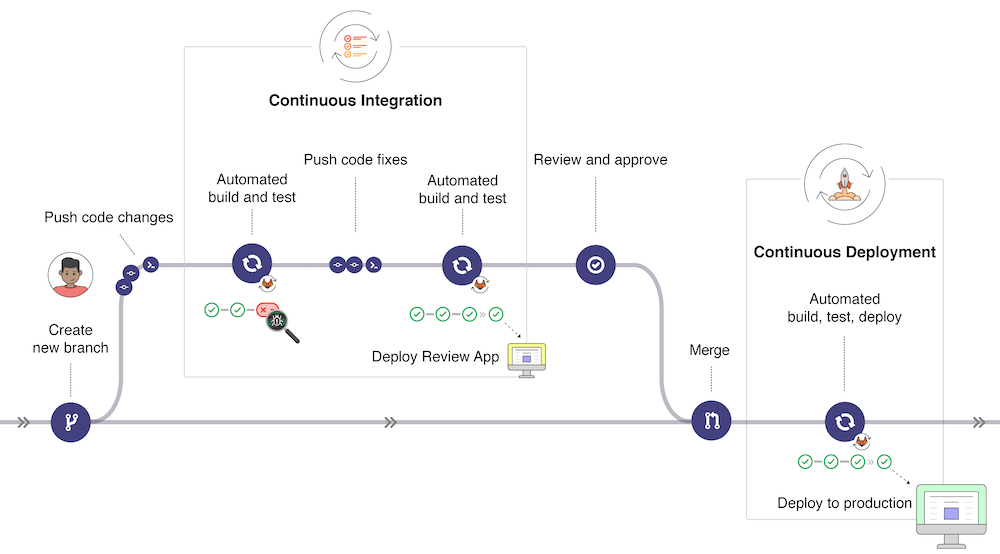
\includegraphics[width=\textwidth]{sources/Gitlab-CI.png}\cite{MG10}
	\caption{Gitlab-CI}
	\label{Continuous integration workflow } {\cite{GLAB1}}
\end{figure}


\subsection{Die Testfälle für unser Projekt}
\paragraph{}
Nachstehend einer Überblick über die Testfälle bei Cypress.
\\
\begin{center}
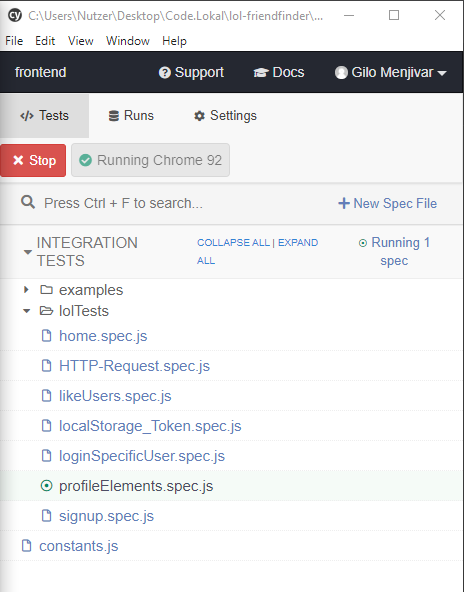
\includegraphics[scale=0.60]{Cy_Test_Cases}\label{fig:Cy_Test_Cases}\\
\textbf{Abbildung \autoref{fig:Cy_Test_Cases}:} Testfälle in Cypress
\end{center}

\begin{center}
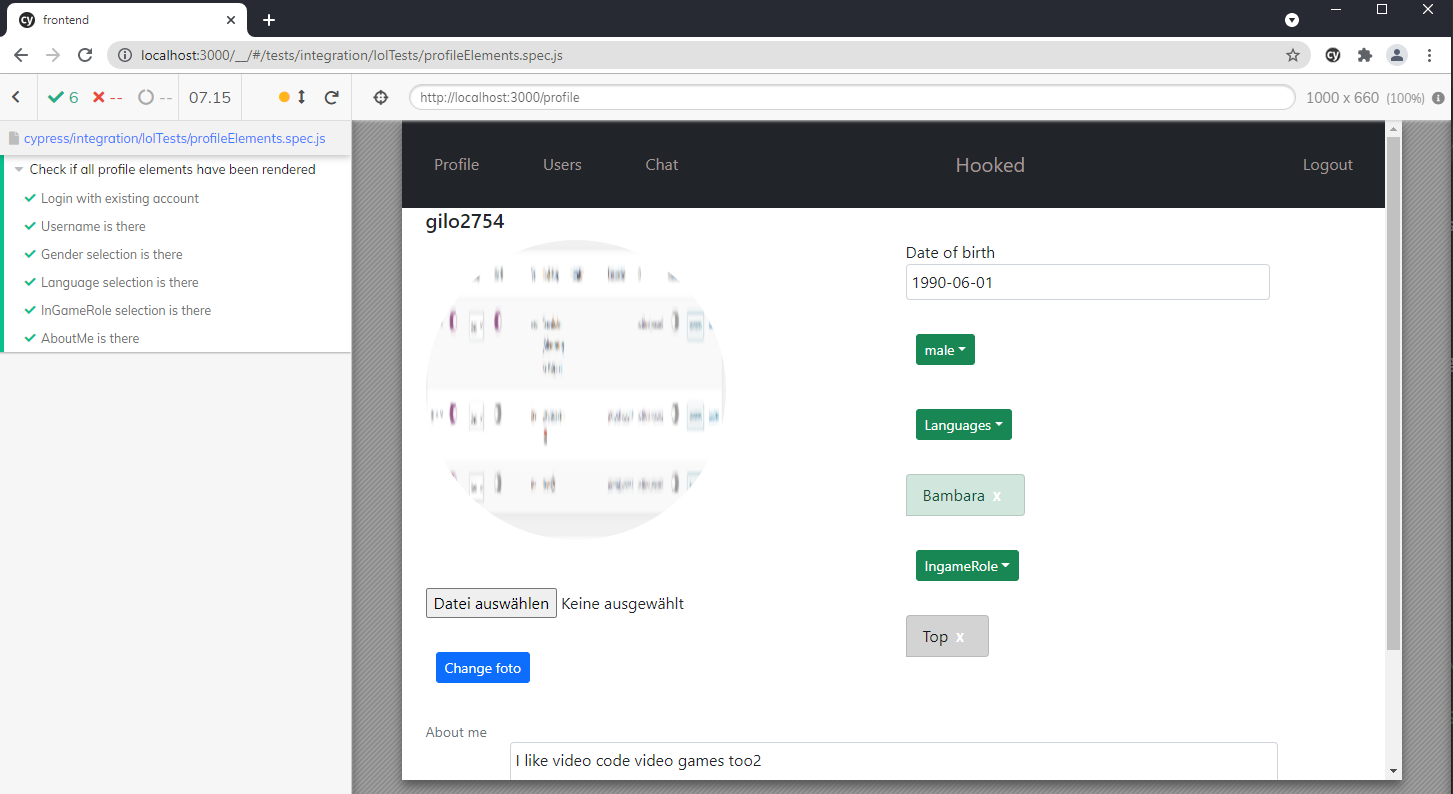
\includegraphics[scale=0.40]{Cy_Test_running}\label{fig:Cy_Test_running}
\textbf{Abbildung \autoref{fig:Cy_Test_running}:} Grafische Darstellung der verschiedenen Tests in Cypress
\end{center}


%Ergebnise der ganzen Testlauf

\subsection{Unit test (Backend)}
To-Do



\begin{comment}
Obwohl das Projekt relativ klein ist, wurde die Wichtigkeit von automatisierten Tests nicht unterschätzt.
\\
Für das Frontend wurden End-to-End Testfälle mit Cypress geschrieben.
Auf diese Weise ist es möglich in Sekundenschnelle festzustellen, ob etwas in unserer Anwendung defekt ist.

Ein Szenario, in dem dies hilfreich ist, ist, wenn eine Unterkomponente in anderen Komponenten verwendet wird.

Durch die Änderung der Unterkomponente kann sich diese in einer unerwünschten Weise verhalten.
\\
Das ist der Fall bei der Komponente AvatarImage.
Dies ist eine Funktionskomponente, die 3 Parameter erhält: Größe des Bildes, Bild-URL und Benutzername.

Zu Beginn des Projekts wurde nicht daran gedacht, die Größe des Bildes über einen Parameter dieser Funktion zu steuern. Im Laufe des Projekts wurde uns klar, dass wir die Logik in diesem Element wiederverwenden konnten.
\\
Innerhalb der Komponente wird geprüft, ob eine URL existiert, und wenn ja, wird das mit dem Link verbundene Bild gezeichnet. Falls es keine URL  angegeben wurde, werden die ersten beiden Buchstaben des Benutzernamens verwendet, um ein Standardsymbol zu erzeugen.

In der aktuellen Version des Codes wird diese Komponente in vier anderen Komponenten wieder verwendet.
Wenn das Projekt weiter wachsen würde, würde auch die Möglichkeit von Fehlern im Code zunehmen. Fehler zu finden, wäre in dem Fall aufwändiger.

Ohne automatisierte Tests, ist manuelles Testing nötig.
\\
Im Anhang 2 befindet sich ein Code-Auszug eines Testfälles End-to-End. 
\end{comment}
%%POSIBLEMENTE ESTE NO ES ELMEJOR EJ PUESTO QUE NO SE ESTA PROBANDO EL TAMANIO LAS IMAGENES EN LAS PRUEBAS DE CYPRESS
%% SIN EMBARGO EL HECHO DE REUTILIZAR LOGICA DE CIERTOS ELEMENTOS ES MUY RELEVANTE Y DEBERIA SER INCLUIDA EN OTRA PARTE %DEL REPORTE
%BUSCAR OTRO EJ. DONDE EL TESTING COBRA MAS RELEVANCIA

